\section{Sequence2Sequence}
% output of LSTM is a non-linear function of the memory, which is the result of the writing and the forget gates. 
Some examples based on the input/output sequence:
\begin{itemize}
    \item One-to-many  - \textit{Image Captioning}: input a single image and get a series or sequence of words as output which describe it. The image has a fixed size, but the output has variable length
    
    \item Many-to-one - \textit{Sentiment Classification/Analysis}: input a sequence of characters or words, e.g., a tweet, and classify the sequence into positive or negative sentiment. Input has variable lengths, output is of a fixed type and size. You accumulate the inputs until the last LSTM, which states an output. 
    \item Many-to-many - \textit{Language Translation}: having some text in a particular language, e.g., English, we wish to translate it in another, e.g., French. Each language has it’s own semantics and it has variable lengths for the same sentence. Can be done in two ways: accumulating the inputs through hidden states or answering directly. The second looks like more natural, but it has some drawbacks: you need that translation can be treat as an aligned process, it works if the input and the outputs are synchronized. Most of Sequence2Sequence model works like the first one.
\end{itemize}{}

The Seq2Seq model follows the classical encoder decoder architecture: at training time the decoder \textbf{does not} feed the output of each time step to the next; the input to the decoder time steps are the target from the training. At inference time the decoder feeds the output of each time step as an input to the next one.

\begin{minipage}{\linewidth}
        \centering
        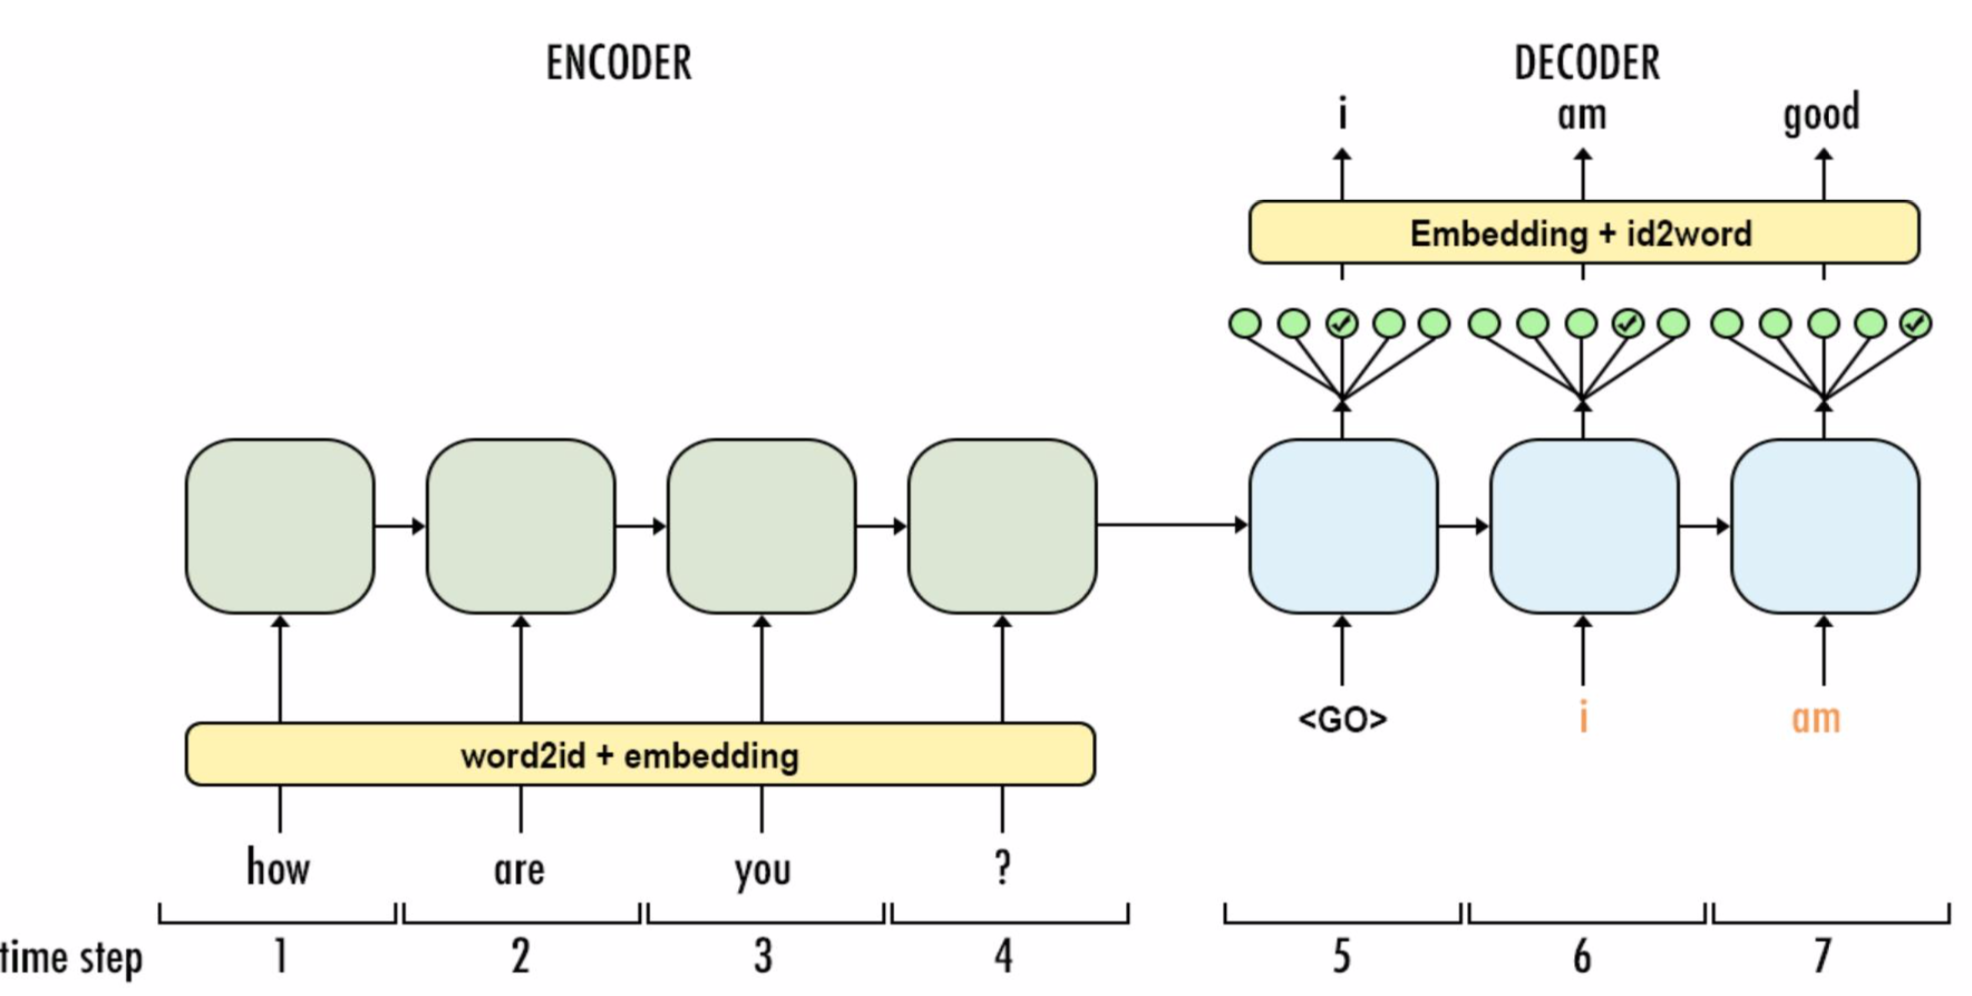
\includegraphics[width=13cm, height=5cm]{images/s2s.png}
        %\captionof{figure}{The model pipeline.}
        %\label{fig:flow_fig}
\end{minipage} \\

%slide 8
%A,B,C is the question, WXYZ is the answer. 
%Once you have learned A B C and you start the output, basing on an special symbol, you output W. Then X is the most likely answer after have been seen A B C D and W. 
%The <eos> is triggered by how you build and modify the state via the answer. 

%slide 9 
At training time, you write the input with no target [the green part]. Only when you input the $<GO>$, you start with the target. Then in order to predict the second target, you feed your network with the previous target.\\
Once the model is trained, you give the input, which ends with $<GO>$ and the model starts to predict the most likely output. As before, once the output is computed, in order to predict the next output, the previous one is given as input. When the network see $<eos>$ is terminates. \\
Each sequence can have different lenght, but you can enforce a maximum length for the output. 
\\
Word Embedding means represent the same word in less sparse representation. The yellow part (the one in the bottom) transforms words into vector , the other yellow part (the one in the top) reverse the process. 
Because of the embedding, the output is the selection among the possible words that it should say as output: usually it is a softmax output among all possible output words. \\

%There are different way to encode into text: bi-grams, tri-grams and so on. This is interesting since tri-grams are less than the number of words in the vocabulary because the pairs of letters. The nice thing is that once you have all the bi-grams or tri-grams you can write all the words in the vocabulary. In principle, also the words that are not in training set. 
Special characters:
\begin{itemize}
    \item[--]$<PAD>$: During training, examples are fed to the network in batches. The inputs in these batches need to be the same width. This is used to pad shorter inputs to the same width of the batch
    \item[--]$<EOS>$: Needed for batching on the decoder side. It tells the decoder where a sentence ends, and it allows the decoder to indicate the same thing in its outputs as well.
    \item[--]$<UNK>$: On real data, it can vastly improve the resource efficiency to ignore words that do not show up often enough in your vocabulary by replace those with this character.
    \item[--]$<SOS>$/$<GO>$: This is the input to the first time step of the decoder to let the decoder know when to start generating output.
\end{itemize}

%slide 10
%Once you have trained your model at runtime, what you do is this. You give the input which ends with GO. So the model start to predict the most likely output. Then this is inputted to the second one and so on. When the network says <eos>, it stops. 
%Each sequence can have different length and you can at runtime enforce a maximum length for the output. 

Sometimes the first best results is not the real best. Usually if you take the second best, the sequence goes better. So you can do what is called \textit{Beam Search} (?): take the first 3 results, then you run three parallel executions. Considering the results of these execution, you choose the best one according to some criteria. \\

%Sometimes the first best is not the best. Usually if you take the second best, usually the sequence goes better. So what you do is what it is called Beam Search [?]: you take the first 3, then you run three parallel execution. Then you get the three more likely and you look three step ahead and you have some criteria to select which will be the best answer. 

Dataset Batch Preparation:
\begin{enumerate}
    \item Sample $batch\_size$ pairs of ($source\_sequence$, $target\_sequence$).
    \item  Append $<EOS>$ to the $source\_sequence$
    \item Prepend $<SOS>$ to the $target\_sequence$ to obtain the $target\_input\_sequence$ and append $<EOS>$ to obtain $target\_output\_sequence$.
    \item  Pad up to the $max\_input\_length$ ($max\_target\_length$) within the batch using the $<PAD>$ token.
    \item Encode tokens based of vocabulary (or embedding)
    \item Replace out of vocabulary (OOV) tokens with $<UNK>$. Compute the length of each input and target sequence in the batch.
\end{enumerate}{}


%slides 11
%Sometimes you have special characters. 

%slides 12 
%This is how you prepare the batch of words. 

%slide 13
In order to compute the error, you have to compute the probability of one character given the state $v$ and the outputs. Given $<S, T>$ pairs, read $S$, and output $T^{\prime}$ that matches $T$: 
$$
\begin{aligned}
p\left(y_{1}, \ldots, y_{T^{\prime}} | x_{1}, \ldots, x_{T}\right) &=\prod_{t=1}^{T^{\prime}} p\left(y_{t} | v, y_{1}, \ldots, y_{t-1}\right) \\
1 /|\mathcal{S}| & \sum_{(T, S) \in \mathcal{S}} \log p(T | S)
\end{aligned}
$$

%You try to minimize the error of the target sequence given the input sequence. To do this, you compute this error as the probability of one character given this state (the encoding) and the previous output: formula

So you can train this model with Cross-Entropy. You can image that each of these networks are softmax over a specific word; you sum the cross-entropy over the sequences and you minimize by the network estimates. So  backpropagate on the cross entropy, trying to get the exact sequence. \\

%slide 14
In general you can stack multiple layer of LSTM: you might have a sort of hierarchical representation. You can perform this embedding hierarchy but through time and then you can have some non-linear transformation (ReLU) at the top. You can also have shortcut connections.\\ 

\paragraph{Bidirectional LSTM}
You can have two level, one goes forward, the other backward through the LSTMs and then you concatenate the LSTMs and you predict the output. The point is: let's assume you want to predict for each word in the sentence if that word is used in positive or negative way in the sentence. If we do it in one direction only, the output depends only on the previous ones. But if the mean of that word change through the sentence, for each word in might be useful what will be after. \\ \\ 

The Sequence2Sequence idea has possible drawbacks: you are compressing long sequences into a vector. It works, backpropagation does not suffer the vanishing gradient, but you can have problem in processing long sequences. The way Seq2Seq is done, the way embedding of sequence into a state and decoding this embedding in another sequence is done, has still some limitation into how much information and how much knowledge or context you can embed into this vector.\\
After a few tests on LSTM people tried to add memory to recurrent neural Networks: it can be achieved in different ways, the most interesting one is the so called \textbf{Neural Turing machine}.

\subsection{Neural Turing machine}
%After a few tests on LSTM people tried to add memory to recurrent neural Networks.
%What does this mean? It can be achieved in different ways, the most interesting one is the so called \textbf{Neural Turing machine}. 
If you remember, in Turing machine you have a infinite
string of symbols
%, reading and writing, 
and you can perform any computation by a series of operations that reads and writes in a sequence from this string. We can do it with the neural network in
the sense that what this recurrent model does is basically storing information in the
memory, reading from it and writing in it. It uses the memory
explicitly 
%(explicit use) 
instead of an encoding of it.\\
So \textbf{Neural Turing Machines} combine a RNN with an external memory bank. \\

\begin{minipage}{\linewidth}
        \centering
        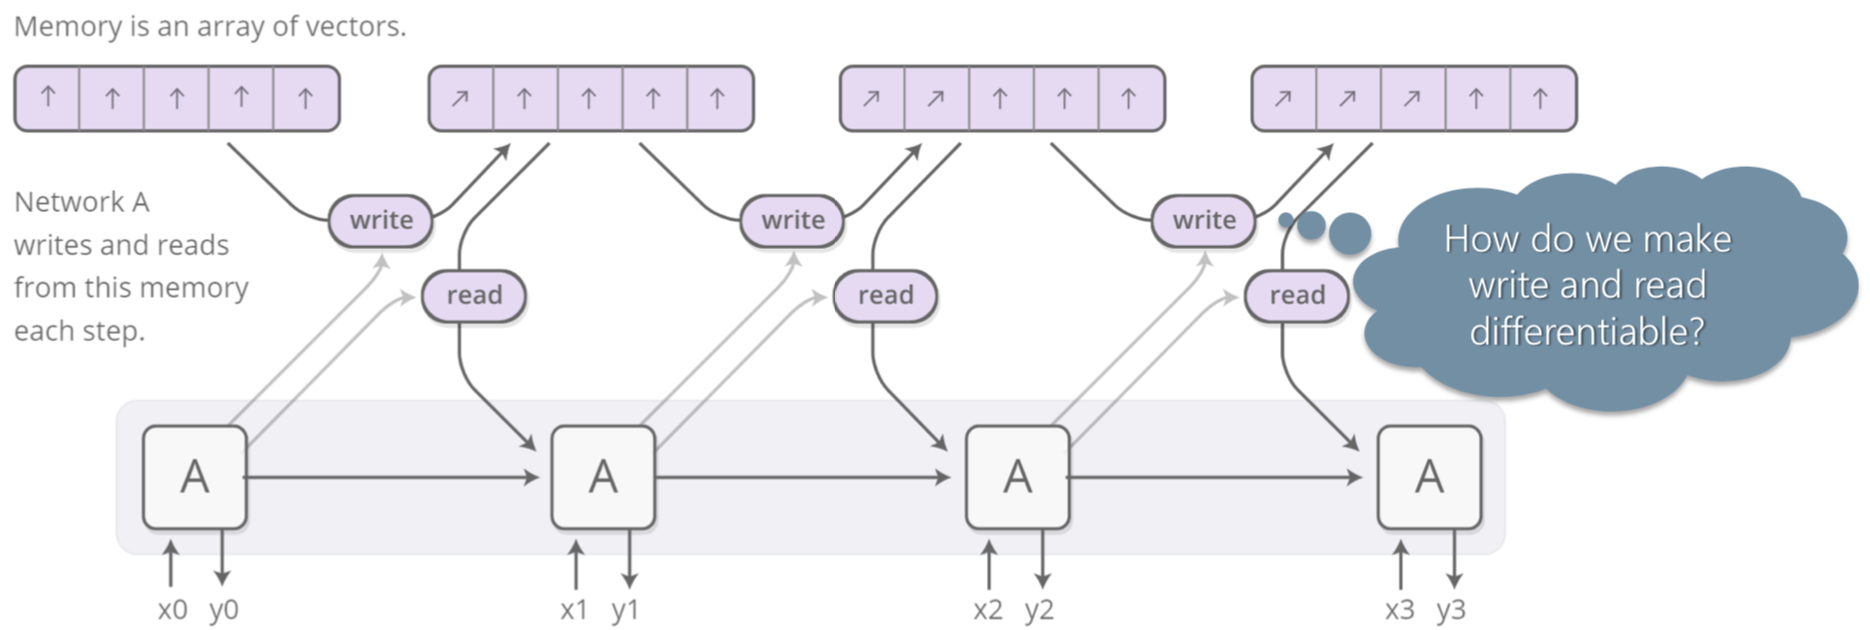
\includegraphics[width=15cm, height=5cm]{images/ntm.png}
\end{minipage} \\ 

I’m using an NTM mostly because the trick used in NTM to read and write for the memory is probably the most interesting part and it’s the same trick upon which we base the attention mechanism. \\
In the figure, you have a network which can write or rewrite the memory given some input; you decide to modify the first cell to store this input and then you read the next step; you get another input and you decide to write the second based on the state of the memory; the same for the third and fourth and so on and so forth. \\
In general, especially when you have long sequences, you would like to partition your memory in states and you would like to use this memory to do things.\\
The problem is that \textit{read} and \textit{write} are \textit{not differentiable} operations.\\
Think about read: reading  means you select one address and extract the cell and only the cell at a specific address; in the same way, writing means you select one address and you change the content of that address.\\
So while writing and reading per se are easy to differentiate, \textit{addressing} is the problem. We would like to learn where to write. Memory addresses are discrete by definition so you should be able to derive
the write and read operation with respect to the address. This
seems a very complex issue which has a very simple solution: \textit{write always everywhere}.\\

Neural Turing Machine challenge:
\begin{itemize}
    \item[--] We want to learn what to write/read but also where to write it
    \item[--] Memory addresses are be fundamentally discrete
    \item[--] Write/read differentiable w.r.t the location we read from or write to
\end{itemize}{}
The solution is: \textit{every step, read and write everywhere, just to different extents} [Attention mechanism]. \\ 
%This way you don’t have to have many recurrent complex things but what you have to do is to learn the sequence of operation read-write-read-write and what to write into. Another mechanism to have memory is somehow not to compress the entire sequence into a single state but to somehow allow the decoding process to \textit{go back} and read what was written in the input, so you have each word in the output depend on each word in the input. This is done with the so called \textbf{attention mechanism} and I would like to discuss the NTM and the attention interfaces. 
%Actually I am more interested in the latter but turns out that introducing NTMs implies an understanding of attention interfaces. 

\begin{minipage}{\linewidth}
        \centering
        \hspace*{-2cm}    
        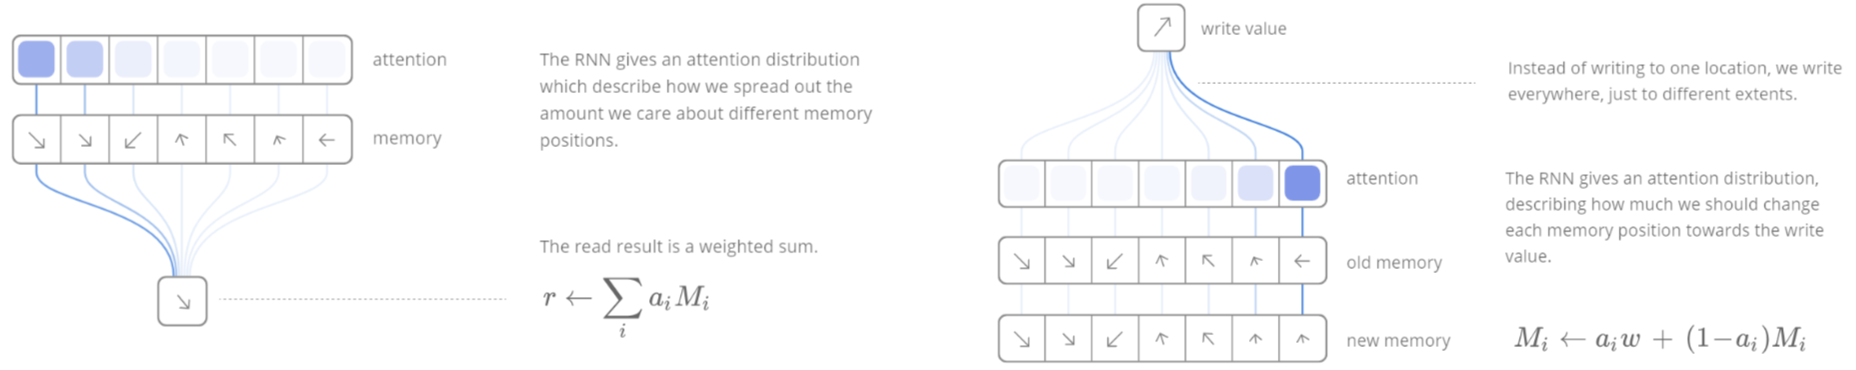
\includegraphics[width=18cm, height=5cm]{images/attention.png}
\end{minipage} \\ \\

%NTM combines recurrent neural networks with memory bank. So basically you have this recurrent neural network, it could be an NTM or a classic recurrent neural network, and make sure you can store enough information in the memory, so you decide that instead of having a set of vectors you have a memory of vectors, so each of these cells contains a vector so that the state would not be one vector summarising the sequence of input so as to average the sequence of input but to be n vectors, and each of them has stored a function of the input and modify this content in a recursive way. For example, assume I get one vector and then I get 7 vectors I don’t need, then a second, then another vector which is the sum of the past 2 vectors combined with the new one; this kind of operation requires to store an input at some point in some place, then store another one and then conditionally get these two, sum the two and put them back. Implementing this, a non linear function of a non linear function of a non linear function, is not necessarily easy to do. 

%Let me get the \textit{translation example}; it’s obvious you want to translate text from one language to another and it’s easy if you have a short context to keep in memory but if you want to memorise 10 pages of text and then translate it exactly from time to time it’s like "okay let me read the first one, let me write some notes here, then let me read the second and write some notes here, then I read the third and write some other notes..." and after I read the notes and I translate the notes instead of writing a single content. So this is a way to increase the memory and the expressivity of the content. This will be very helpful also with respect to NTM and Sequence to Sequence encoding.  I’m using an NTM mostly because the trick used in NTM to read and write for the memory is probably the most interesting part and it’s the same trick upon which we base the attention mechanism. 

%So let’s see here you have a network which can write or rewrite the memory so basically you have some input, you decide to modify this cell to store this input and then you read the next step, you get another input and you decide to write the second based on the state of the memory, then the third and fourth and so on and so forth. In general, especially when you have long sequences, you would like to partition your memory in states and you would like to use this memory to do things.

%If you think about the reversed string or reversed text, it becomes very easy this way. If you want to write a string in reverse order then it’s more complex because the context has to store the \textit{sequence} of words you have used plus the \textit{order} you have used, and if the model is a reversed model string, you cannot imagine that in the training set you have all the strings and the reversed ones. So basically, to learn an LSTM reversible string is much more difficult than to learn an NTM reversible string; what you have to do is write from left to right when you see the go symbol (non so perché lo dica) read from right to left and you have reversed it, so it’s easier and quite straightforward to implement reversed string, so writing and learning algorithms is easier. 

%The problem is that read and write are not differentiable operations. Think about read, reading  you select one address and extract the cell and only the cell at a specific address, write you select one address and you change the content of that address.
%So while writing and reading per se are easy to differentiate, \textit{addressing} is the problem. We would like to learn where to write.

%Memory address are discrete by definition so we should be able to derive the write and read operation with respect to the address. This seems a very complex issue which has a very simple solution: \textit{write always everywhere}.

%How much you decide to write depends on the input. In each step, I write everything but mostly in some cells, so it means that based on my input I will write in this cell and not in that one. It’s a sort of associative writing but in principle at each step I could write everywhere. Think about LSTM gates, the idea is the same, in each cell you decide where and what to write, here the gate is over the entire memory and you decide on all the cells ‘on this I write on this I don’t’. So the idea is to have an \textbf{attention mechanism}: basically your data will tell you where to write, so that it puts your attention on specific cells. You have your memory and this is the ‘read’ so you say you have to read from this cell so you put attention here. 

How much you decide to write depends on the input. In each step, I write everything but mostly in some cells, so it means that based on my input I will write in a cell and not in another one. It’s a sort of \textit{associative writing} but in principle at each step I could write everywhere. \\
Thinking about LSTM gates, the idea is the same: in each cell you decide where and what to write; here the gate is over the entire memory and you decide on all the cells to which cell to write or not to write.\\
%‘on this I write on this I don’t’. 
So the idea is to have an \textbf{Attention mechanism}: basically your data will tell you where to write, in order to put your attention on specific cells. \\
In the left part of the Figure, you have your memory and a ‘read’: you want to read from a particular cell, thus you put attention there. \\
Two types of attention: 
\begin{itemize}
    \item[--] \textbf{Content-based attention}: searches memory and focus on places that match what they're looking for
    
    \item[--] \textbf{Location-based attention}: allows relative movement in memory enabling the NTM to loop
\end{itemize}{}

\begin{minipage}{\linewidth}
        \centering
        \hspace*{-2cm}    
        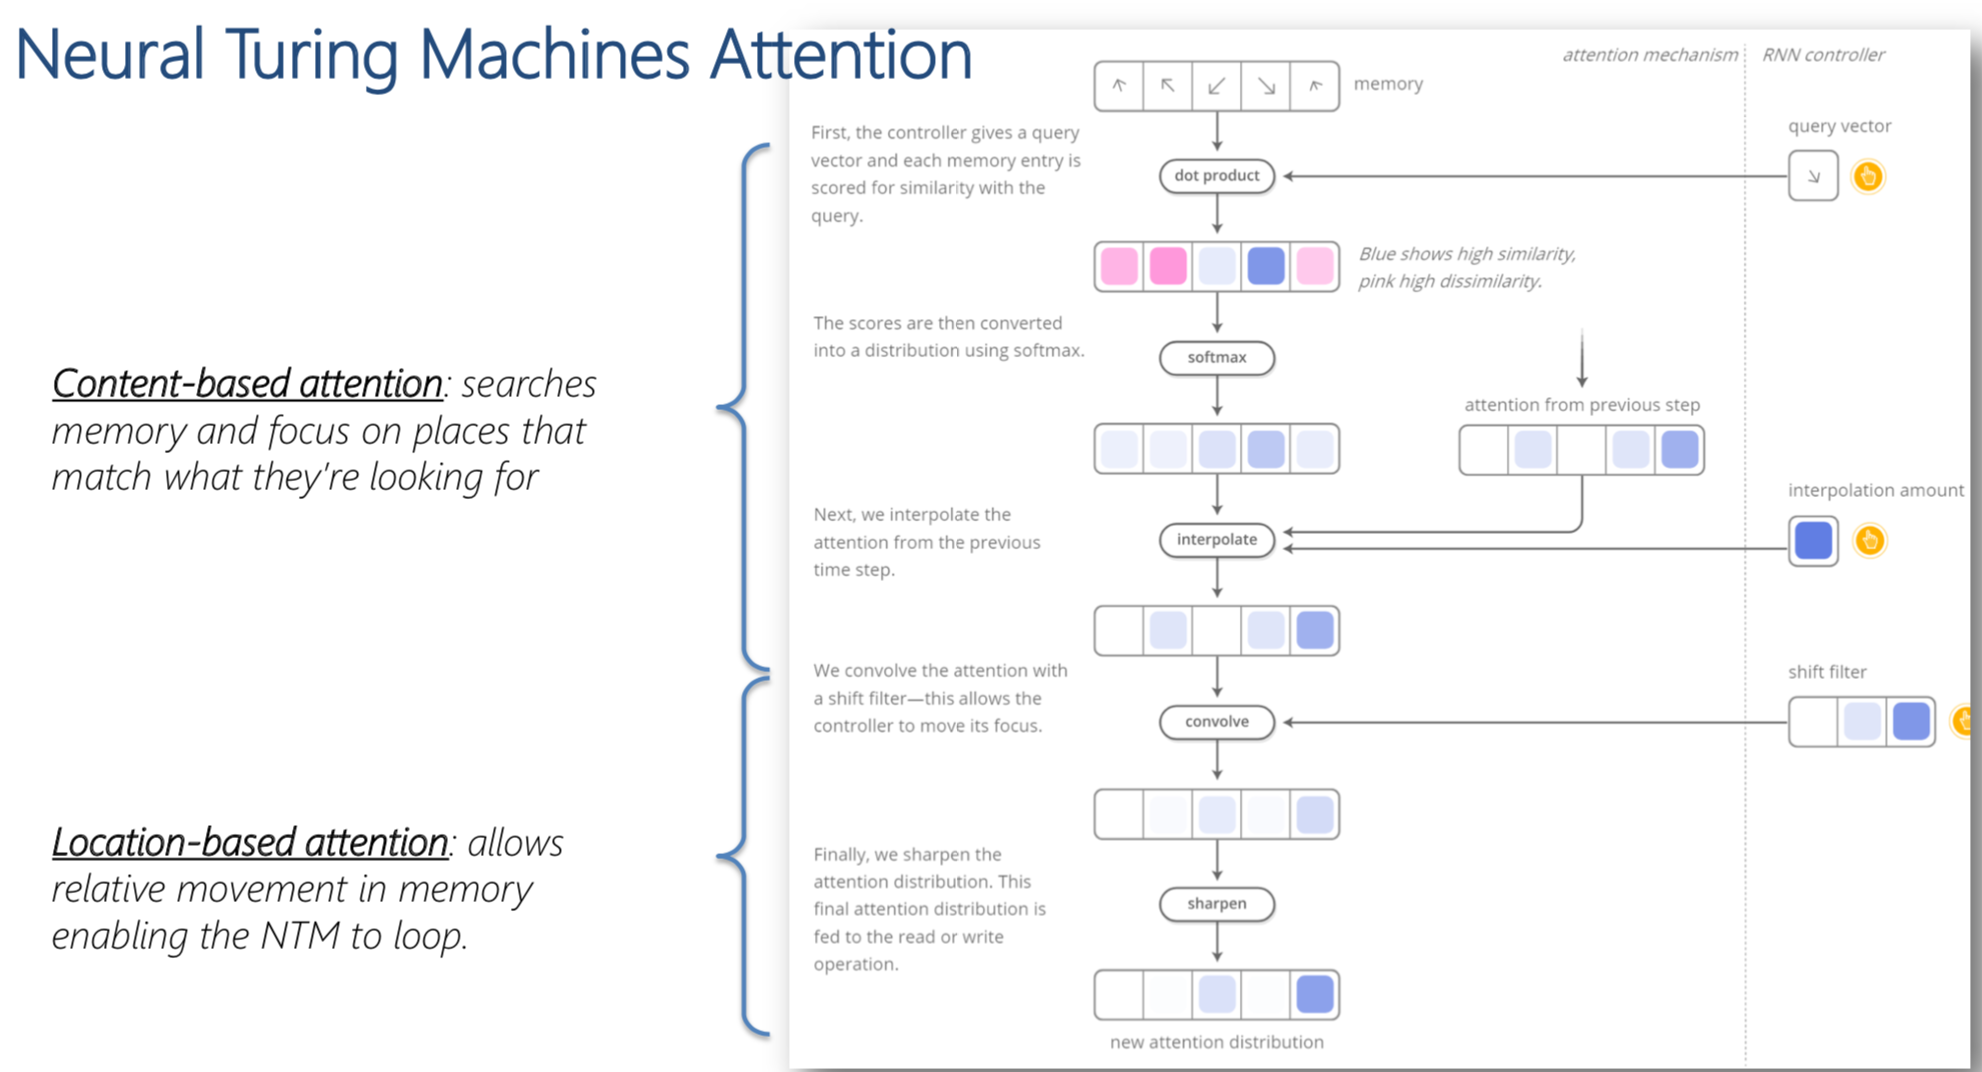
\includegraphics[width=14cm, height=8cm]{images/attention_example.png}
\end{minipage} \\ \\

Think about having a softmax output: 
%\begin{center}
%    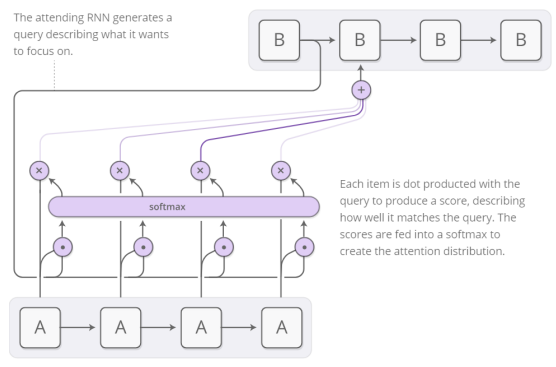
\includegraphics[width=0.6\textwidth]{images/attentionsoft.PNG}\par
%\end{center}
%it has some peaks which are very close to 1, so basically if this is the softmax of a neural network, given a certain input you can select with this softmax which cell you’re gonna read; what happens is that the reading would be the weighted average where the weights are the softmax weights of your entire reading. Because the softmax is very selective (it’s a normalised exponential function) you would read mostly from one or two or three cells, and if for some reason you would read from 3 because you can still retrieve multiple cells from the memory and the interesting part is that you can derive this because it is nothing but the product between the memory, which is nothing more than a set of vectors, and the attention which is a softmax and it's differentiable. Each item is thus weighted with the query response to produce a score.

Basically, given a certain input you can select with this softmax which cell you’re gonna read; what happens is that the reading would be the weighted average where the weights are the softmax weights of your entire reading. \\
Because the softmax is very selective (it’s a normalised exponential function - it's almost everywhere equal to 0) you would read mostly from one or two or three cells 
%,and if for some reason you would read from 3 because you can still retrieve multiple cells from the memory 
and the interesting part is that you can derive this because it is nothing but the product between the memory, which is nothing more than a set of vectors, and the attention, which is a softmax and it is differentiable.\\
Each item is thus weighted with the query response to produce a score.\\


%So if you have 1 0 0 0, this way you only replace the memory cell. Let’s assume you have 0,5 here and 0,5 here, you merge this cell with the new value, this cell with the new value, and at the end the part is left unchanged. You didn’t really select those 2, you wrote everywhere but since this softmax is almost everywhere equal to 0, its almost like selecting some specific cells. Once you learn the trick it’s pretty simple. Now you can jump multiple vector stored and you don’t have necessarily each of them to depend on the history of the network, plus you can have attention memory which depends on the input. SO let’s put this into an entire network.


%Let’s assume that you have your memory and some input vector. This input vector to some extent should trigger the cell in the memory you want to write into. So for instance you might decide this query vector is retrieving which cells are most similar to this input. So you would change the memory cells which are more similar to this input. Based on this you have a similarity pick, then a softmax layer on this similarity pick, which will select which one is the current attention, the current cell you want to put attention on. Sometimes the attention depends not only on the current input but also on the previous input, so let’s assume you want to learn to look around so my attention goes first there, now it should go there again but since I have already looked there i’ll go there (forse è un diverso there) because you want to move or interpolate your attention mechanism to somehow have a local smoothness. You have this interpolation which is a parameter between the old attention and te new attention, this parameter will tell you how much to shift your attention from one timestamp to the other, then you have this attention that can have a shift .. so you only move the focus, you don’t jump, you chase the focus instead of jumping from one place to another, you sharpen because you want the minimum amount of cells. SO after these operation you have decided which are the cells to write in. This is a complex implementation of what I said before. 
Based on the input, you have a softmax on the memory and the output gets changed based on this memory. The softmax is driven by the input, so it’s a content-based attention, and once you have retrieved the most similar area in the memory, you have a sort of location-based mechanism 
%not to jump from one location to another 
and this location mechanism allows you to move from one area to another.\\ 

%Now, this is what I wanted to talk about for Turing Machines, I don’t really want to get into this sort of different architectures, but 
What is interesting and relevant of NTM is the idea that you can \textbf{focus on a PART} of your memory: this is \textbf{Attention}!\\
%It’s better than LSTM in remembering long sentences, they can learn how to look in sequences, to sort or reverse numbers, something which is not easy in lstm because you have to encode the order in one single-context vector while here you don’t need to do that because the memory sorts things, and there are many improvements on Neural Tuning machines, but, besides this improvements, what I’m interested in is Attention. Probably the most relevant outcome of NTM in these models is the idea that you can avoid mixing things by storing them and to focus or weight these memory cells.


\subsubsection{Attention Mechanism in Seq2Seq Models}
So people realized that the attention mechanism could have been an interesting add-on for the Sequence to sequence model I was talking about before. \\

%So people realized that the attention mechanism could have been an interesting add-on for the Sequence to sequence model I was talking about before. Why? Let me make an example so make it clear. Lets consider a set of sequences with a set of inputs and a set of outputs, the decoder (the sequence generator) has the goal of generating this sequence of output starting from the input which is the context, and this is the summary of the sequence. If you do a standard vanilla seq2seq model, which is what we have discussed so far, your decoder is conditioned on the initial state which is the last state of the encoder (slide 23). For a short or medium-length input it works quite well, but if you have long sequences what happens is that you might have a problem at this point because you have squeezed all the information into one single vector and you might want to do it a little bit more flexible and more structured as you were doing with memories. So the trick is I don’t have a memory but I have a past, so instead on condition only on this state, I would have to condition this on the output of this on the output of this, I condition my sequence of words based on the words that had in the (event). 

Considering the sequential dataset $
\left\{\left(\left(x_{1}, \dots, x_{n}\right),\left(y_{1}, \dots, y_{m}\right)\right)\right\}_{i=1}^{N}
$, the decoder role is to model the generative probability: $P(y_1, ..,y_m | x)$.\\
In "vanilla" seq2seq models, the decoder is conditioned initializing the initial state with last state of the encoder. That works well for short and medium-length sentences; however, for long sentences, becomes a bottleneck.\\
Let's use the same idea of Neural Turing Machines to get a differentiable attention and learn where to focus attention.\\ 

\begin{minipage}{\linewidth}
\centering
\hspace*{-2cm}    
\begin{minipage}{9cm}
  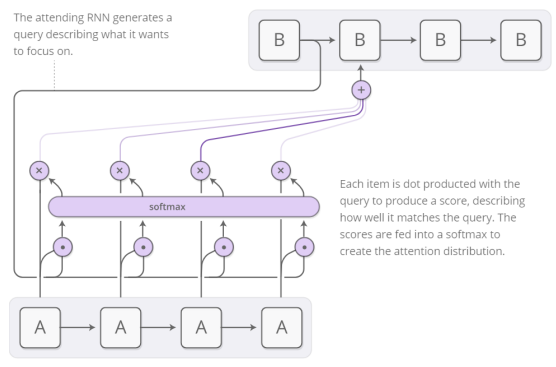
\includegraphics[width=9cm, height=7cm]{images/attentionsoft.PNG}
  %\captionof{figure}{A figure}
  %\label{fig:test1}
\end{minipage}%
\begin{minipage}{10cm}
  \centering
  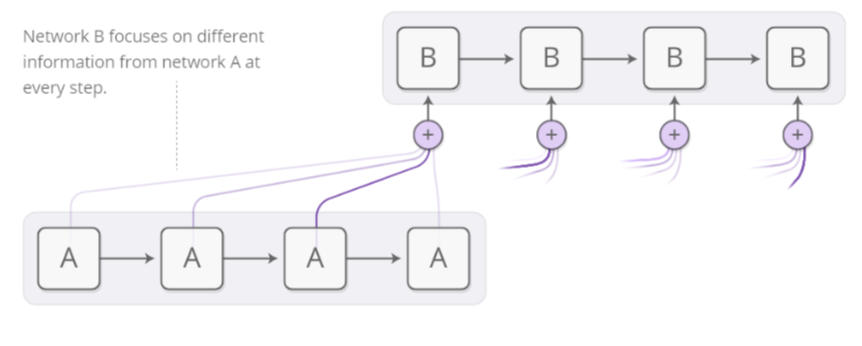
\includegraphics[width=10cm, height=4cm]{images/attentionsoft_right.png}
  %\captionof{figure}{Another figure}
  %\label{fig:test2}
\end{minipage}
\end{minipage}\\ \\

Attention distribution is usually generated with content-based attention.\\
Each item is thus weighted with the query response to produce a score. Scores are fed into a softmax to create the attention distribution

Attention function maps query and set of key-value pairs to an output. \\
Output computed as a weighted sum of the values, where the weight assigned to each value is computed by a compatibility function:


\begin{enumerate}
    \item Compare current target hidden state $\boldsymbol{h_t}$ with source states $\boldsymbol{h_s}$ to derive attention 
    $$
    \operatorname{score}\left(\boldsymbol{h}_{t}, \overline{\boldsymbol{h}}_{s}\right)=\left\{\begin{array}{l}
    {\boldsymbol{h}_{t}^{\top} \boldsymbol{W} \overline{\boldsymbol{h}}_{s}} \\
    {\boldsymbol{v}_{a}^{\top} \tanh \left(\boldsymbol{W}_{1} \boldsymbol{h}_{t}+\boldsymbol{W}_{2} \overline{\boldsymbol{h}}_{s}\right)}
    \end{array}\right.
    $$
    
    \item Apply the softmax function on the attention scores and compute the attention weights, one for each encoder token
    $$
\alpha_{t s}=\frac{\exp \left(\operatorname{score}\left(\boldsymbol{h}_{t}, \overline{\boldsymbol{h}}_{s}\right)\right)}{\sum_{s^{\prime}=1}^{S} \exp \left(\operatorname{score}\left(\boldsymbol{h}_{t}, \overline{\boldsymbol{h}}_{s^{\prime}}\right)\right)}
$$
    
    \item Compute the context vector as the weighted average of the source states
    $$
    \boldsymbol{c_t} = \sum_{S} \alpha_{ts}\boldsymbol{ \overline{\boldsymbol{h}}_s}
    $$
    \item Combine the context vector with current target hidden state to yield the final attention vector
    $$
\boldsymbol{a}_{t}=f\left(\boldsymbol{c}_{t}, \boldsymbol{h}_{t}\right)=\tanh \left(\boldsymbol{W}_{c}\left[\boldsymbol{c}_{t} ; \boldsymbol{h}_{t}\right]\right)
$$
\end{enumerate}{}

\begin{minipage}{\linewidth}
\centering
\hspace*{-2cm}    
\begin{minipage}{9cm}
  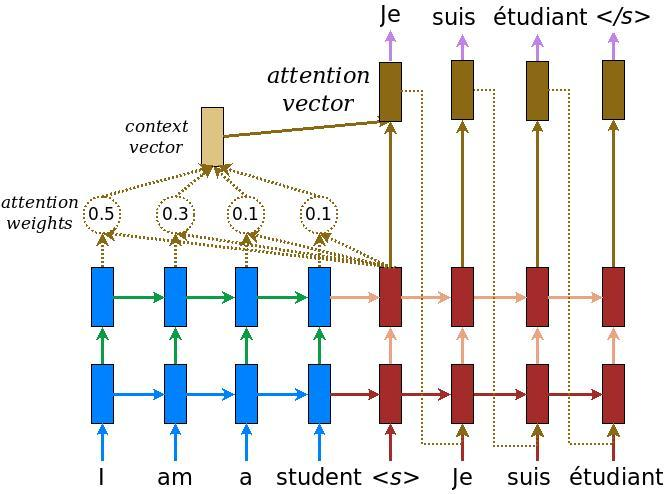
\includegraphics[width=9cm, height=7cm]{images/attention_mechanism.jpg}
  %\captionof{figure}{A figure}
  %\label{fig:test1}
\end{minipage}%
\begin{minipage}{10cm}
  \centering
  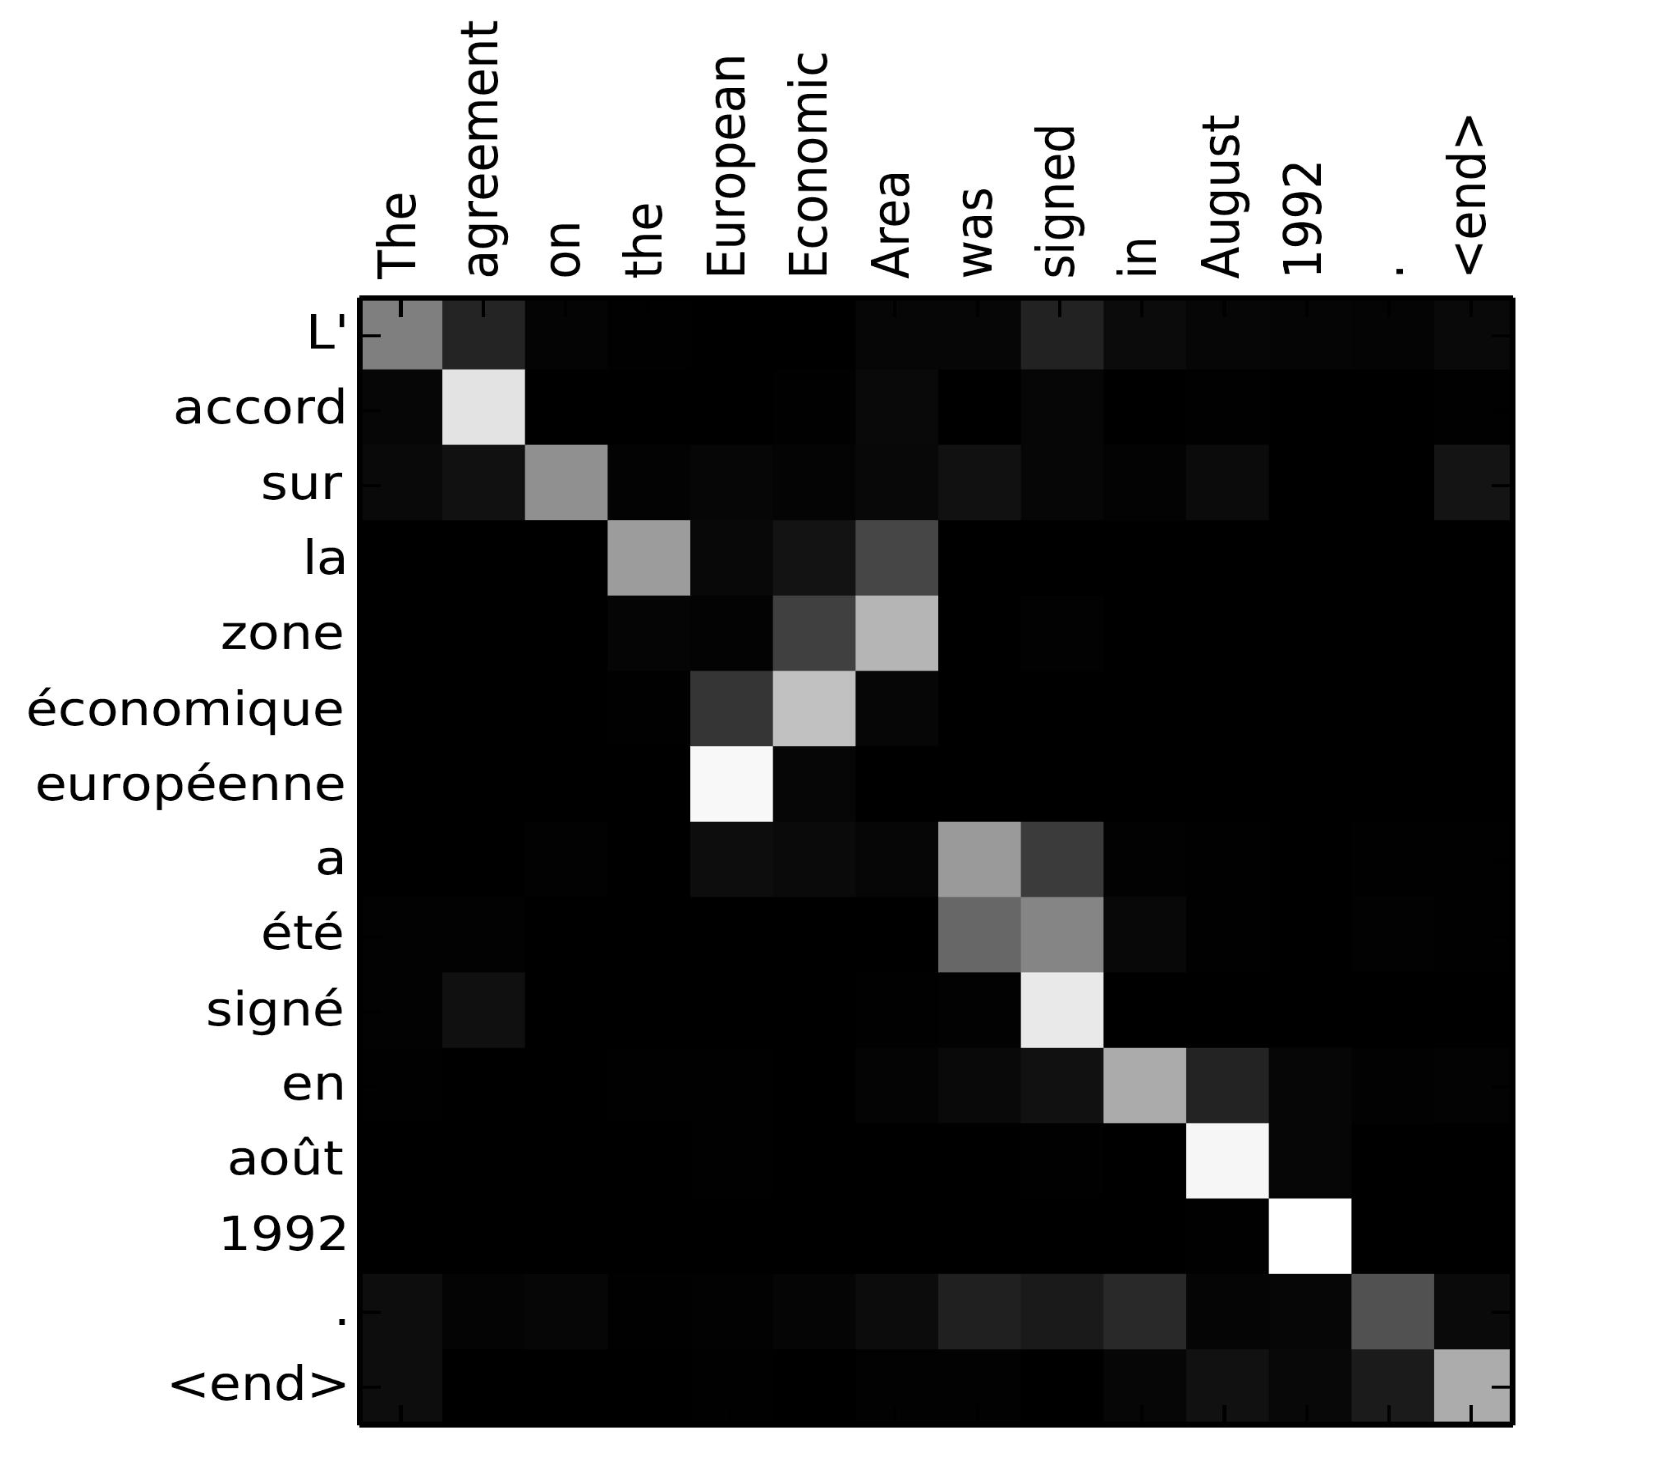
\includegraphics[width=9cm, height=8cm]{images/bahdanau-fig3.png}
  %\captionof{figure}{Another figure}
  %\label{fig:test2}
\end{minipage}
\end{minipage}\\ \\


%SO basically if I translate ‘ I AM A’ if I have to translate the next word I would like to look at what’s written here, it’s like a memo. (24:16) So basically the idea is to have a sort of network mechanism, when you decode you are allowed to use input as the memory, so you start by looking at the sort of summary of the sentence but then you have to go back and say what was that for? Because this is available to your decoder, you have the input and the entire sequence and after looking after initialising this sequence you can add to the current state some input which was the past encoding so it’s like this: you have the first word, you encode it, you get the last word, you encode it, and then at each step you have a sort of attention mechanism based on current decoder which retrieves the last word, so to predict the next word you use the current state plus you retrieve like the reading mechanism from the past encoding a sort of more focused context. It’s like saying okay I get the point on the meaning of the text, I start writing and then from time to time when you are writing you look around you scatter around the previous text to say like ‘okay this I wrote this I wrote this I wrote’. With the images (quella sopra) this becomes clear immediately, think about capturing, you want to capture this ‘the cat is on’ and you look below the ‘cat’ and you say ‘table’, you focus on the part of the image which is always available and is relevant at that point. You do this starting from the central pick, the center, you would never describe the table is below the cat, you start from the cat which is in the center. So you have a sequence which is this internal state which tricks input in generating this (new sequence). Let’s see a simulation of this attention mechanism. 
%As you can see, you do exactly what’s written here, you do these replicas and so on and so forth, but you have also some connection here which are weighted, it’s a weighted sum with weights which are based on the content of the previous state. So the idea is the attention is a sort of content based (addressee? address?), so based on this value you retrieve the information in one sense. Based on your current state here you can retrieve the past, then you build a context vector which is not the very last but it’s based on attention, then you move forward and your attention changes, then you move forward again and you attention changes and so on. You keep the input as a memory. At this point you get I AM A STUDENT, the attention is on the second word, AM and JE but the trick is that you look back, at each step you know on which word you are putting your attention.

%So the idea is you have the current target in the state with the source state and you have a sort of attention, compare this with this and you use this to compare which is the most relevant out of these. You have some possible ways of computing the score. Given your final context you can retrieve a score between this context and the past. For instance, what is the most relevant score in the past based on this sequence, and then you build a context vector by mixing.. so from this core you built an attention mechanism, it’s not particularly complex in this case, then once you have the score between this and all the hidden states, a softmax, you build a context vector as the weighted sum of all these (contexts), so you use the last context to retrieve what word was the most relevant state and you build a new state as a new context, so you put your attention in generating the sentence, for instance you start here: the first one would be ‘I’ so you put a set of weights, your attention is on ‘I’ and ‘Je’, then you get Je, you change this state, you look here what is the most interesting word to go here, and it’s this so you get the hidden representation on AM, so basically by doing this you can jump back and forth, this jump is related to the current context, it’s related to the input and the output. How to retrieve is.. by doing this basically what happens is these two matrixes are used to compute ——- (sembra dica ‘are learned’) and this (———) so to know how to put your attention based on the history based on the train set on the input. Then you combine your hidden with this context, so you keep, so it’s just an add-on on the classic Sequence2Sequence and you go on forward. What you can do is at each time look at this vector and at the weights on this vector. 

The Figure on the right represents the \textbf{Alignment matrix}, used to visualize attention weights between \textit{source} and \textit{target} sentences. \\
For each decoding step, i.e., each generated target token, describes which are the source tokens that are more present in the weighted sum that conditioned the decoding. \\
We can see attention as a tool in the network’s bag that, while decoding, allows it to pay attention on different parts of the source sentence.

\begin{minipage}{\linewidth}
        \centering
        \hspace*{-2cm}    
        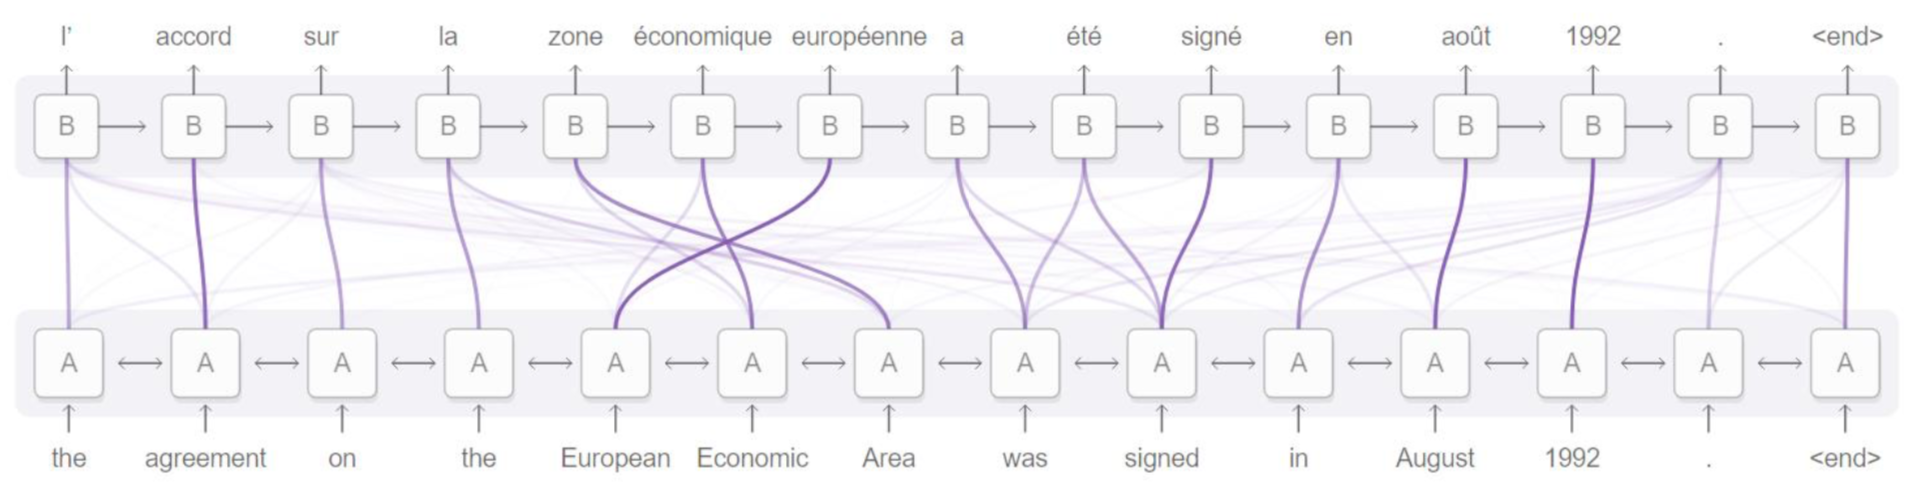
\includegraphics[width=17cm, height=5cm]{images/attention_example_french.png}
\end{minipage} \\

Attention allows processing the input to pass along information about each word it sees, and then for generating the output to focus on words.
Attention can be used in different scopes:
\begin{itemize}
    \item[--] Translation
    \item[--] Voice Recognition: attention allows one RNN to process the audio and then have another RNN skim over it, focusing on relevant parts as it generates a transcript.
    \item[--] Image Captioning: a CNN processes the image, extracting high-level features. Then an RNN runs, generating a description of the image based on the features. As it generates each word in the description, the RNN focuses on the CNN interpretation of the relevant parts of the image.
\end{itemize}{}

\subsubsection{Attention in Respose Generation - Chatbots}
Chatbots can be defined along at least two dimensions:
\begin{itemize}
    \item \textbf{Core Algorithm}:
    \begin{itemize}
        \item \textit{Generative}: encode the question into a context vector and generate the answer word by word using conditioned probability distribution over answer’s vocabulary. E.g., an encoder-decoder model.
        
        \item \textit{Retrieval}: rely on knowledge base of question-answer pairs. When a new question comes in, inference phase encodes it in a context vector and by using similarity measure retrieves the top-k neighbor knowledge base items.
    \end{itemize}{}
    
    \item \textbf{Context Handling}:
    \begin{itemize}
        \item \textit{Single-turn}: build the input vector by considering the incoming question. They may lose important information about the history of the conversation and generate irrelevant responses
        $$ {(q_i, a_i)}$$
        
        \item \textit{Multi-turn}: the input vector is built by considering a multi-turn conversational context, containing also incoming question  
        $$
        \left\{\left(\left[q_{i-2} ; a_{i-2} ; q_{i-1} ; a_{i-1} ; q_{i}\right], a_{i}\right)\right\}
        $$
    \end{itemize}{}
\end{itemize}{}

Vinyals and Le, 2015 and Shang et al., 2015 proposed to directly apply sequence to sequence models to the conversation between two agents:
\begin{enumerate}
    \item The first person utters “ABC”
    \item The second person replies “WXYZ”
\end{enumerate}{}

Generative chatbots use an RNN and train it to map “ABC” to “WXYZ”: we can borrow the model from machine translation; a flat model simple and general; Attention mechanisms apply as usual. \\

\textbf{Generative Hierarchical Chatbots} The idea could be concatenating multiple turns into a single long input sequence, but this probably results in poor performances. \\
LSTM cells often fail to catch the long term dependencies within input sequences that are longer than 100 tokens.\\
No explicit representation of turns can be exploited by the attention mechanism.\\

Xing et al., in 2017, extended attention mechanism from single-turn response generation to a hierarchical attention mechanism:
\begin{itemize}
    \item Hierarchical attention networks (e.g., characters $\rightarrow$ words $\rightarrow$ sentences)
    \item Generate hidden representation of a sequence from contextualized words
\end{itemize}{}

(Hierarchical Generative Multi-turn Chatbots - Hierarchical Document Classification guardare le slide) \\

\textbf{Attention is all you need} Having seen attention is what makes things working you start wondering: 
\begin{itemize}
    \item[--] Sequential nature precludes parallelization within training examples, which becomes critical at longer sequence lengths, as memory constraints limit batching across examples.
    
    \item[--]Attention mechanisms have become an integral part of compelling sequence modeling and transduction models in various tasks. Can we base solely on attention mechanisms, dispensing with recurrence and convolutions entirely?
    
    \item[--] Without recurrence, nor convolution, in order for the model to make use of the order of the sequence, we must \textbf{inject} some information about the relative or absolute position of the tokens in the sequence.
\end{itemize}{}
There has been a running joke in the NLP community that an \textbf{LSTM with attention} will yield \textit{state-of-the-art} performance on any task.
Attention is built upon RNN, .. The \textbf{Transformer} breaks this assumption!

\subsubsection{Transformer}
\begin{wrapfigure}{r}{7cm}
    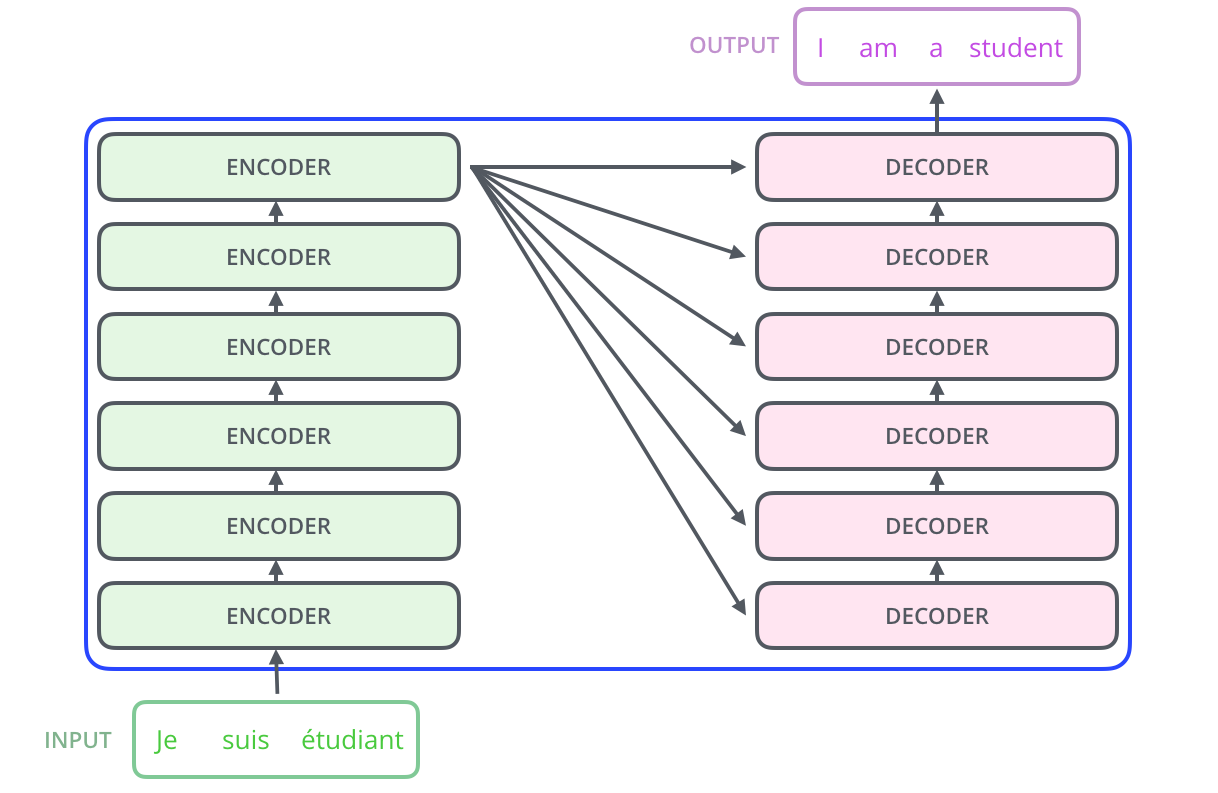
\includegraphics[width=7cm]{images/The_transformer_encoder_decoder_stack.png}
\end{wrapfigure} 

In a Transformer model we can distinguish an encoding component, a decoding component, and connections between them. \\
The Encoders are all identical in structure (yet they do not share weights). Each one is broken down into two sub-layers:
\begin{enumerate}
    \item \textit{Self-Attention}: a layer that helps the encoder look at other words in the input sentence as it encodes a specific word
    \item \textit{Feed Forward Neural Network}: The outputs of the self-attention layer are fed to a feed-forward neural network. The exact same feed-forward network is independently applied to each position [\textbf{Position-wise Feed-Forward NN}]
\end{enumerate}{}
The Decoder has the following layer:
\begin{enumerate}
    \item \textit{Self-Attention}: as before
    \item \textit{Encoder-Decoder Attention}: helps the decoder focus on relevant parts of the input sentence
    \item \textit{Feed Forward Neural Network}: as before
\end{enumerate}{}

We begin by turning each input word into a vector using an embedding algorithm. The embedding only happens in the bottom-most encoder. \\
After embedding the words in our input sequence, each of them flows through each of the two layers of the encoder. Here we begin to see one key property of the Transformer, which is that the word in each position flows through its own path in the encoder. There are dependencies between these paths in the self-attention layer. The feed-forward layer does not have those dependencies. So the self-attention layer, in some way, stores the dependencies of inputs, while the Feed Forward is treated as 'independent' for each input.\\

\begin{wrapfigure}{r}[2cm]{8cm}
    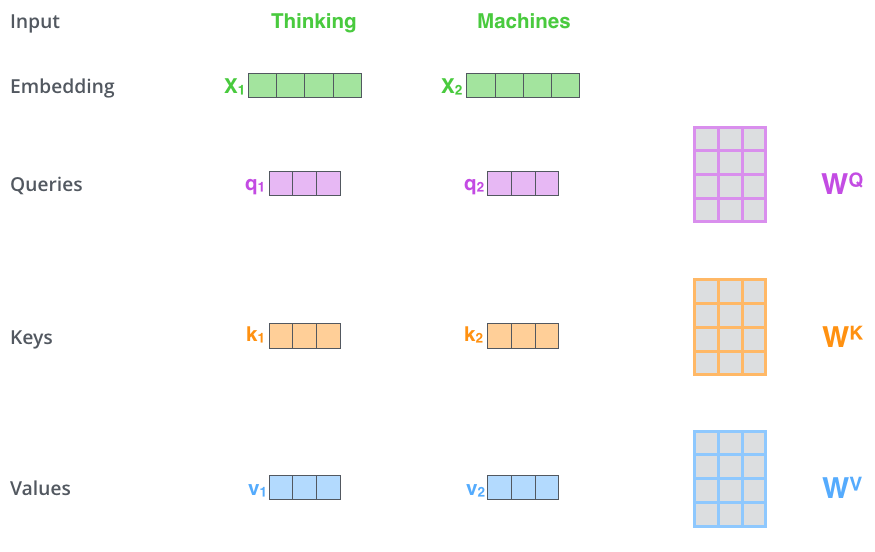
\includegraphics[width=8cm]{images/transformer_self_attention_vectors.png}
\end{wrapfigure}

\textbf{Scaled Dot-Product Attention}\\
The \textbf{first step} in calculating self-attention is to create three vectors from each of the encoder’s input vectors: a \textit{Query vector}, a \textit{Key vector}, and a \textit{Value vector} [they are abstraction that are useful for the calculus]. These vectors are created by multiplying the embedding by three matrices that we trained during the training process. \\
Multiplying $x_1$ by the $W^Q$ weight matrix produces $q_1$, the "query" vector associated with that word. We end up creating a "query", a "key", and a "value" projection of each word in the input sentence. \\

The \textbf{second step} in calculating self-attention is to calculate a score: we need to score each word of the input sentence against this word. The score determines how much focus to place on other parts of the input sentence as we encode a word at a certain position. The score is calculated by taking the dot product of the query vector with the key vector of the respective word we’re scoring: so if we’re processing the self-attention for the word in position \#1, the first score would be the dot product of $q_1$ and $k_1$. The second score would be the dot product of $q_1$ and $k_2$. \\

The \textbf{third} and \textbf{forth steps} are to divide the scores by the square root of the dimension of the key vectors $\sqrt{d_k}$: this leads to having more stable gradients.\\
Then pass the result through a softmax operation. Softmax normalizes the scores so they’re all positive and add up to 1. \\

The \textbf{fifth step} is to multiply each value vector by the softmax score: the intuition here is to keep intact the values of the word(s) we want to focus on, and drown-out irrelevant words (by multiplying them by tiny numbers like 0.001, for example) \\

The \textbf{sixth step} is to sum up the weighted value vectors. This produces the output of the self-attention layer at this position (for the first word). \\

At the end the \textit{Attention} can be expressed as $$ Z = 
\text { Attention }(Q, K, V)=\operatorname{softmax}\left(\frac{Q K^{T}}{\sqrt{d_{k}}}\right) V
$$

\begin{wrapfigure}{r}[2cm]{5cm}
    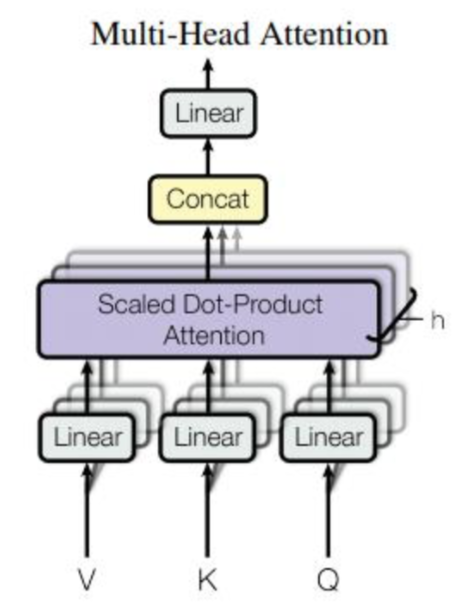
\includegraphics[height=5cm]{images/multihead.png}
\end{wrapfigure}

\textbf{Multi-head Attention} If we do the same self-attention calculation we outlined above, just $h$ different times with different weight matrices, we end up with $h$ different Z matrices. \\
The feed-forward layer is not expecting $h$ matrices – it’s expecting a single matrix (a vector for each word). So we concat the matrices then multiple them by an additional weights matrix $W^0$ (which was trained jointly with the model). \\
The result would be the Z matrix that captures information from all the attention heads: this matrix is sent to the FNN.\\

\textbf{Positional Encoding} One thing that’s missing from the model as we have described it so far is a way to account for the order of the words in the input sequence. To address this, the transformer adds a vector to each input embedding. These vectors follow a specific pattern that the model learns, which helps it determine \textbf{the position} of each word, or the distance between different words in the sequence. The intuition here is that adding these values to the embeddings provides meaningful distances between the embedding vectors once they’re projected into Q/K/V vectors and during dot-product attention. \\ \\

To sum up, a Transformer model is made out of:
\begin{itemize}
    \item Scaled Dot-Product Attention
    \item Multi-head Attention
    \item Position-wise Feed-Forward Networks
    \item Embeddings and Softmax
    \item Positional Encoding
\end{itemize}{}
Self-Attention has $O(1)$ maximum path length; when $n < d$, Self-Attention has lower complexity per layer.


%So this is called Alignment Matrix (slide 27) and provides you with this alpha value as a function of the input, the sequence. So in the beginning the attention is on ‘L’ACCORD SUR LA ZONE’.. ehm reading French is still torturing (LOL).. so let’s read it this way ‘THE AGREEMENT ON THE EUROPEAN ECONOMIC AREA WAS SIGNED IN AUGUST 1992’, you want to translate this in French so you don’t have to read it (lol) so basically the first term you want to put your attention on is THE and you get this (L’). Now that you have written this, the second term you want to put your attention is AGREEMENT, then you translate it (ACCORD), then the next word you put attention on is ON (SUR) and then THE (LA) and now your attention ‘European economic area’ it’s interesting because in English you have the typical reversion (inversion magari) between name and adjective, so you want to focus on AREA which is economic of Europe. If you think of translating this into Italian, the first word you want to translate is AREA, not European. And the same is in French. Next time I will translate into Italian so I know how to read it properly *laughs* some other people was probably more proficient in French than me. So you see that now the attention based on the past is on this term because the way you do it is more clear if you translate from French to English. Let’s do it in Italian LA ZONA ECONOMICA EUROPEA: LA is an article, it’s female, and it refers to a noun; the next noun is ZONA, so I have to put my attention on this; and then I put my attention on the adjective and then this (prima ‘economica’, poi‘europea’). But in English they get reversed so by this mechanism you see that you can look at some groups of words A E’TE’ = WAS SIGNED, in August... this is related to the mere alignment of text. SO you see that you are able to focus on different parts of the sentence so most of the time the attention is on a group of letters which are useful to predict which is the right. So here you see you try, you kind of learn the alignment between the text and more interesting is that this very nice demo but I won’t speak about this demo we will come back on this later, you can do this with images as well: so for instance, let’s assume you want to produce caption, this same mechanism, let me do it this way.. when you have a sentence.. if you do captioning here you have the image, right? (forse sta disegnando qualcosa alla lavagna) and here you have the encoding or the cnn output of the image. You start with the first term and based on that now only a part of the image is relevant, you focus your attention on part of the image. Then when you have processed that, you focus your attention on another part of the image. And so you have the shift of attention. How you do a mask, i already told you how you do an attention mechanism with —— masking instead of.. right here you have a matrix which multiplies your image and removes some features and keeps others. Yes? (domanda di qualcuno su alpha.. let’s go to the images then it’s easier. SO basically what happens is that you have a frisbee and this object. So if in the training set you have an image with a frisbee and an image without it you see that when you do the propagation, this part of the image is the most relevant to predict the word frisbee with respect to this one. So if you want to compute what is the derivative of this word with (in) respect to this image, the derivative is maximum if you are here. And if you want to say, okay for each pixel, which should I use, which I shouldn’t, the maximum is when the softmax tells you to use this and not use this, and it’s maximum the correlation. Now every time you have a frisbee in the image, the masking is this, is selecting the area where you want to put attention, and then it’s strengthening it. Now you have used this area, it sees the next mask is based on the previous one (if you remember the neural tuning machine) that happen is that then you have already talked about the frisbee so you shift your attention elsewhere so basically your focus here is first on the woman, then what is she doing, the frisbee, then you shift your attention elsewhere. So basically you see that when you add.. so here what is the first thing you look at is the dog but then what’s beneath and then you look around, so the sequence, you have already talked about the dog, so your attention is shifting. In the last 5 minutes let me show, let’s hope it works... first thing, let’s see if I can reach this website or not.. if not it’s not a problem but.. so it’s not a real problem, it means that we have to used from a computer connected to the network or with a VPN.. so I have updated the vpn.. and it works.. so this is a problem because I wanted you to use it from your laptop but you need to be on the vpn as well.. so basically the idea is that you can make any questions about any of these images, pick one of the images you prefer, let’s see.. let’s do this one okay. So the goal is to have.. ask me something: what is he doing? Now the interesting part (the first time it takes some time cause it has to load), so the interesting part is what is he doing means that it’s processing this image, conditioning, and now it’s answering to the question, and the question should put attention on the image so that it will look around. Now there are two algorithms (quando più avanti chiede le risposte runna entrambi e prende 2 risposte generate da quanto capisco), one is a state of the art algorithm which has been trained this way this is a.. I think a —-(MS qualcosa) Dataset, it has been trained with 3000 possible answers, and based on my question on this image, the algorithm will select one of the answers or the most likely answer. SO there is a big bias so if what is he doing, if half of the dataset is about skating, it will answer skating and it will appear to be very nice.. the algorithm was developed by your colleague and it does not have any predefined set of answers, that’s why the title is open-ended question answering, so it is based on a very powerful language generating model so it should be able to answer questions that were not those originally planned by the other —-. So the answer the algorithm is saying is skateboarding, now let’s see your colleague what is it saying.. skateboarding! What is nice is that what is the algorithm you’re paying attention to, so here the attention is WHAT (so on the bench)- IS - HE.. so you see that based conditioned on the input you shift DOING.. then it start SKATE- BOARDING, you see skateboarding is big —- it’s a language model that in principle could write sentences that are not based on single word but also composite and so on. For instance if we ask on this question WHAT IS ON THE BENCH, again you get an answer, the classical bags and here you see what I was saying: the question is general, so it’s not looking at the image because there is no bag, but.. here may be one but it’s very.. let’s see the another one.. girl and phone *laughs* and this is clearly not.. I mean.. long hair girl clearly.. one is the most common. So let’s ask another question WHAT IS THE BOY WEARING? So the answer is.. Shorts, which are not.. Shirt and shorts, which is wrong! But WHAT COLOR IS THE BOY SHIRT? The answer is blue. Now here you can see where they are looking.. no one is looking at the.. they are looking at the trousers. It’s very difficult to understand.. let me try to get another image where we can make more interesting questions.. every time it loads random images.. this I have already.. *laughs*. Now the interesting part is WHAT IS HE DOING? This is interesting. He’s sitting and..—- (non capisco cosa dice ma tutti ridono). Another.. WHAT VEGETABLE IS IT? Broccoli is correct, broccoli which is correct, and you see here what it was looking at.. so WHAT IS THIS? —— so we can ask what is on the ground? ‘Vegetables’ and ‘plants and bananas’ *lols* plants and bananas is a classical answer, the dataset is quite biased.. let me..